\newpage
\section{Analiza problemu}		%2

\subsection{Zastosowanie struktur danych i wzorców projektowych}
Dwukierunkowa lista wiązana jest jedną z fundamentalnych struktur danych w informatyce. Znajduje szerokie zastosowanie w sytuacjach wymagających częstych operacji wstawiania i usuwania elementów w dowolnym miejscu kolekcji, bez konieczności realokacji całej pamięci (co wyróżnia ją na tle zwykłych tablic). Jest powszechnie wykorzystywana m.in. w:
\begin{itemize}
    \item Mechanizmach cofania operacji (\textit{Undo/Redo}) w edytorach tekstów czy programach graficznych.
    \item Implementacji pamięci podręcznej typu LRU \cite{stroustrup}(\textit{Least Recently Used}).
    \begin{figure}[!htb]
    	\begin{center}
    		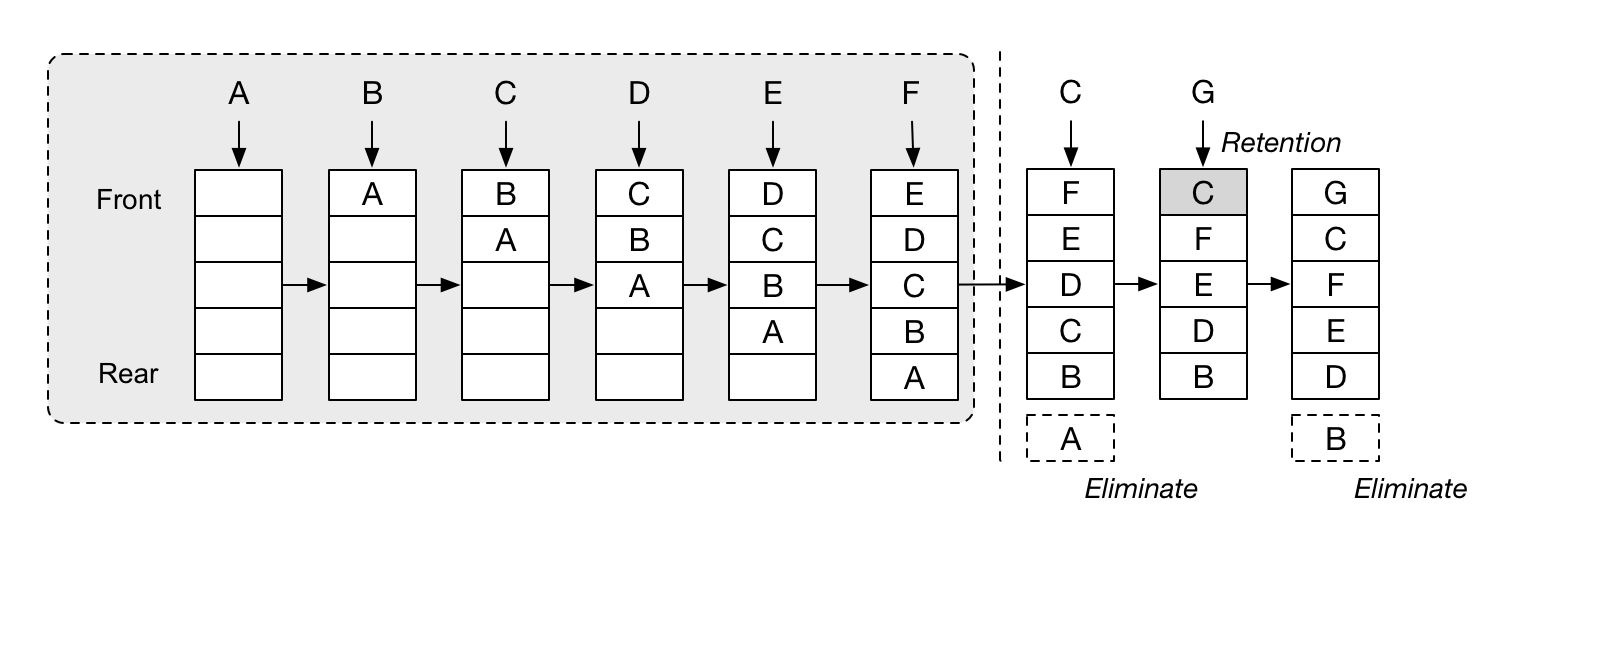
\includegraphics[width=0.8\linewidth]{rys/lru-algorithm.png}
    		\caption{Przykładowy algorytm LRU}
    		\label{rys:rysunek003}
    	\end{center}
    \end{figure}
    \item Zarządzaniu oknami i historią nawigacji w przeglądarkach internetowych.
\end{itemize}

W ramach projektu zastosowano również wzorce projektowe: \textbf{Wzorzec Iterator} (ułatwiający sekwencyjny dostęp do elementów listy bez ujawniania jej wewnętrznej reprezentacji) oraz \textbf{Wzorzec Fabryki} (centralizujący proces tworzenia nowych obiektów węzłów).

\subsection{Sposób działania programu i algorytmów}
Program zarządza dynamiczną alokacją pamięci za pomocą wskaźników łączących poszczególne węzły (\texttt{Node}). Każdy węzeł przechowuje wartość całkowitą oraz dwa wskaźniki: na element następny (\texttt{next}) oraz poprzedni (\texttt{prev}). 

Główne algorytmy zaimplementowane w projekcie obejmują:
\begin{enumerate}
    \item \textbf{Dodawanie elementów (\texttt{addFront}, \texttt{addBack}, \texttt{addAtIndex}):} Alokacja nowego węzła w pamięci za pomocą fabryki, a następnie odpowiednie przepięcie wskaźników ``głowy'' (\texttt{head}), ``ogona'' (\texttt{tail}) oraz sąsiadujących węzłów.
    \item \textbf{Usuwanie elementów (\texttt{removeFront}, \texttt{removeBack}, \texttt{removeAtIndex}):} Wyszukanie elementu, zmiana powiązań wskaźników w celu pominięcia usuwanego węzła, zwolnienie pamięci funkcją \texttt{delete} oraz aktualizacja rozmiaru listy.
    \item \textbf{Przechodzenie przez iteratory:} Klasa pomocnicza \textit{ListIterator} zarządza aktualnym wskaźnikiem i przeciąża operatory inkrementacji (\texttt{++}), umożliwiając bezpieczne przeglądanie zawartości.
\end{enumerate}

\subsection{Przykład działania algorytmu wstawiania}
Aby zilustrować działanie algorytmu wstawiania, przeanalizujmy ręcznie proces dodawania elementu o wartości $20$ na sam początek listy, w której znajduje się już jeden element o wartości $10$.

\begin{enumerate}
    \item \textbf{Stan początkowy:} 
    Lista posiada wskaźnik \texttt{head} skierowany na węzeł $[10]$. Węzeł $[10]$ ma \texttt{prev = nullptr} oraz \texttt{next = nullptr}.
    
    \item \textbf{Krok 1 (Utworzenie węzła):} 
    Fabryka tworzy nowy węzeł o wartości $20$ (\texttt{newNode}). Jego wskaźniki ustawione są domyślnie na \texttt{nullptr}.
    
    \item \textbf{Krok 2 (Przepięcie wskaźników):} 
    \begin{itemize}
        \item Nowy węzeł wskazuje swoim polem \texttt{next} na dotychczasową głowę: \texttt{newNode->next = head;} (czyli węzeł $[10]$).
        \item Dotychczasowa głowa aktualizuje wskaźnik wsteczny: \texttt{head->prev = newNode;} (węzeł $[10]$ wskazuje na nowy węzeł).
        \item Wskaźnik \texttt{head} całego obiektu listy zostaje zaktualizowany i wskazuje teraz na \texttt{newNode} ($[20]$).
    \end{itemize}
    
    \item \textbf{Stan końcowy:} 
    Otrzymujemy spójną listę dwukierunkową: \texttt{head} $\leftrightarrow [20] \leftrightarrow [10] \leftrightarrow$ \texttt{tail}.
\end{enumerate}

\subsection{Opis narzędzi wspierających projekt}
W procesie tworzenia i testowania oprogramowania wykorzystano nowoczesne narzędzia inżynieryjne:
\begin{itemize}
    \item \textbf{Git oraz GitHub:}\cite{git_scm, github_docs}System kontroli wersji, który umożliwił śledzenie zmian w kodzie źródłowym, bezpieczne testowanie nowych funkcji na oddzielnych gałęziach (\textit{branchach}) oraz archiwizację projektu.
    \item \textbf{Microsoft Visual Studio oraz MSBuild:} Środowisko programistyczne dostarczające kompilatora MSVC (narzędzie wiersza poleceń \texttt{cl}), służące do budowania i uruchomienia kodu napisanego w języku C++.
    \item \textbf{Doxygen:}\cite{doxygen_site} Narzędzie do automatycznego generowania dokumentacji technicznej na podstawie ustandaryzowanych komentarzy zawartych w kodzie źródłowym.
    \begin{figure}[!htb]
    	\begin{center}
    		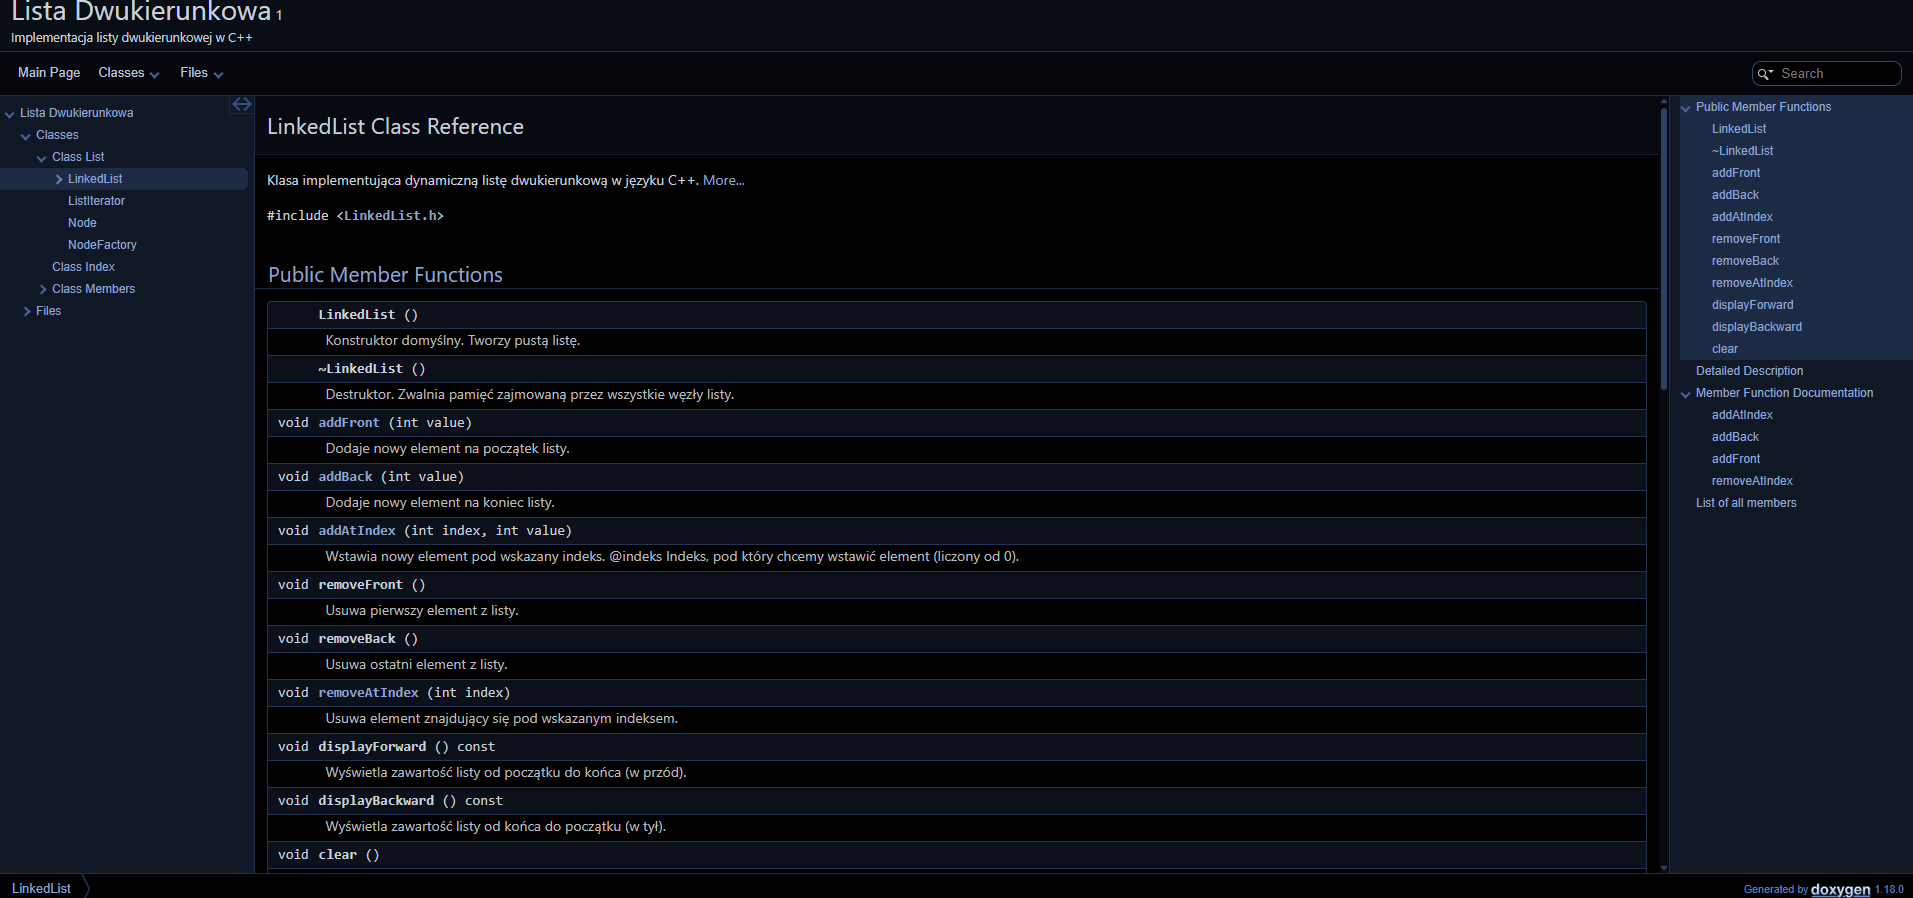
\includegraphics[width=0.8\linewidth]{rys/doxy.png}
    		\caption{Strona HTML wygenerowana przez program}
    		\label{rys:rysunek003}
    	\end{center}
    \end{figure}
\end{itemize}